\documentclass[a4paper, 11pt]{report}

\usepackage[margin=1in]{geometry}

\usepackage[hidelinks]{hyperref}

\usepackage[utf8]{inputenc}
\usepackage[english,greek]{babel}
%\usepackage[LGR]{fontenc}

\usepackage{graphicx}
\graphicspath{ {images/} }

\usepackage[usenames, dvipsnames]{color}
\definecolor{mygray}{gray}{0.6}

%make pdflatex output copy-and-paste-able
\input{glyphtounicode}
\pdfgentounicode=1

%shortcuts
\newcommand{\gr}{\selectlanguage{greek}}
\newcommand{\en}{\selectlanguage{english}}

\begin{document}
\begin{center}{\small ΠΑΝΕΠΙΣΤΗΜΙΟ ΠΑΤΡΩΝ - ΤΜΗΜΑ ΜΗΧΑΝΙΚΩΝ Η/Υ ΚΑΙ ΠΛΗΡΟΦΟΡΙΚΗΣ }	
\end{center}

{\Large \noindent\textbf{Λειτουργικά Συστήματα}
\hfill \textbf{Άσκηση 2}}

\begin{flushright}
	\textbf{Εργασία Φοιτητή:}\\
	Δαμιανός Ντούμη - Σιγάλας, 6157\\
	\texttt{\en \href{mailto:nsigalas@ceid.upatras.gr}{nsigalas@ceid.upatras.gr}\gr}
\end{flushright}

\setlength{\parskip}{10pt}%

\vspace{-0.5cm}

\noindent \textbf{Υλοποίηση των \en mysh1 \gr και \en mysh2 \gr}

Ο κώδικας που αφορά το \en \texttt{mysh1} \gr και το \en \texttt{mysh2} \gr είναι κοινός καθώς το δεύτερο αποτελεί προεκτασή της πρώτης περίπτωσης. Επομένως τα δύο αρχεία \en (\texttt{mysh1.c, mysh2.c}) \gr έχουν πανομοιότυπο περιεχόμενο. Η λογική που ακολουθήθηκε περιγράφεται παρακάτω.

Αρχικά, εμφανίζεται το \en prompt \gr στην οθόνη (\texttt{\$ }) αναμένοντας την είσοδο του χρήστη, η οποία αποτελείται από το όνομα του ζητούμενου προγράμματος ή εντολής και πιθανόν διαφορές παραμέτρους που εξειδικεύουν την λειτουργία του. Έπειτα η είσοδος χωρίζεται σε κομμάτια με βάση τον κενό χαρακτήρα, δημιουργώντας έτσι έναν πίνακα αλφαριθμητικών σε κάθε θέση του οποίου έχουμε και από ένα μέρος της εντολής.

Στη συνέχεια ελέγχεται αν η είσοδος αποτελεί κάποιο \en built-in command \gr του \en shell \gr (στην περίπτωσή μας \en \texttt{exit} \gr και \en \texttt{cd}\gr) ή είναι απαραίτητη η κλήση κάποιου άλλου προγράμματος ώστε να πραγματοποιηθούν οι κατάλληλες ενέργειες και να εκτελεστεί το αντίστοιχο πρόγραμμα.

Στην περίπτωση που ο χρήστης επιθυμεί την εκτέλεση ενός τρίτου προγράμματος τότε με χρήση της \en fork \gr η διεργασία γονέας (δηλαδή το \en shell \gr μας) δημιουργεί και αναμένει την εκτέλεση μιας διεργασίας παιδιού η οποία αναλαμβάνει να εκτελέσει ένα στιγμιότυπο του ζητούμενο προγράμματος (με χρήση του \en system call \texttt{execvp}\gr).

Το πρόβλημα που αντιμετώπισα σε αυτό το σημείο αφορά την σωστή διαχείριση της εισόδου του χρήστη καθώς το μέγεθος και ο αριθμός των παραμέτρων μιας εντολής δεν είναι γνωστός. Επομένως απαιτείται η δυναμική εκχώρηση μνήμης σχετικά με την δέσμευση ενος \en array of strings\gr, σε κάθε θέση του οποίου αποθηκεύεται και ένα μέρος του \en user input\gr, χωρισμένο με βάση τον κενό χαρακτήρα. Η λογική αυτή υλοποιείται στη συνάρτηση \en \texttt{char** parse\_command();} \gr η οποία αναλαμβάνει να φέρει το αρχικό αλφαριθμητικό σε μορφή κατάλληλη για παράμετρο της \en \texttt{execvp}\gr.

\noindent \textbf{Υλοποίηση των \en mysh3 \gr και \en mysh4 \gr}

Σε αυτά τα δύο \en shells \gr προστίθεται η υποστήριξη του \en piping \gr. Όταν μεταξύ δύο εντολών παρεμβάλλεται ένας \en vertical bar \gr χαρακτήρας τότε η εντολή που βρίσκεται στα αριστερά ανακατευθύνει την έξοδο της στο άκρο εγγραφής ενός \en pipe \gr ώστε η δεξια εντολή να ανακατευθύνει την είσοδο της στο άκρο ανάγνωσης του ίδιου \en pipe \gr λαμβάνοντας τα δεδομένα που έγραψε σε αυτό η πρώτη.

\begin{center}
	\vspace{-0.25cm}
	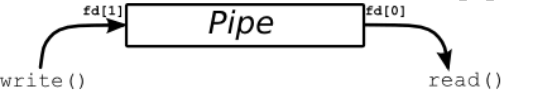
\includegraphics[scale=0.25]{pipe}\\ \vspace{-0.25cm}
	\en\texttt{leftmost command | \textcolor{mygray}{(...)} | rightmost command}\\ \gr
\end{center}

Αφού χωρίσουμε την είσοδο με βάση τα \en vertical bars\gr, κάθε \en token \gr που προκύπτει πρέπει να χωριστεί με βάση το κενό και να έρθει σε μορφή κατάλληλη για την \en\texttt{execvp}\gr. Στην περίπτωση του \en \texttt{mysh3} \gr που γνωρίζουμε εκ των προτέρων ότι θα έχουμε μόνο δύο εντολές (επομένως είναι σταθερός ο αριθμός των εντολών και άγνωστο το πλήθος των παραμέτρων κάθε εντολής) η διαδικασία είναι παρόμοια με αυτή που περιγράφεται στα πρώτα δύο \en shells\gr. Στο \texttt{\en mysh4\gr} το πλήθος των \en pipes \gr που αναμένουμε δεν είναι γνωστό. Έτσι πέρα από το άγνωστο πλήθος παραμέτρων κάθε εντολής το πρόγραμμα θα πρέπει να διαχειρίζεται και άγνωστο πλήθος εντολών. Για τον σκοπό αυτό δημιουργείται ένας πίνακας τύπου \en \texttt{char***} \gr κάθε θέση του οποίου αποθηκεύει δείκτες σε \en array of strings (\texttt{char**}) \gr καθένα από τα οποία περιέχει μία εντολή με την μορφή που περιγράφεται παραπάνω.  

Για παράδειγμα με είσοδο \en\texttt{"ls -l -a | sort | wc -w"} \gr o πίνακας θα έχει την μορφή:

\en 
\noindent\texttt{
char** cmd[3] = \{
		\{"ls", "-l", "-a", NULL\},
		\{"sort", NULL\},
		\{"wc", "-w", NULL\}
	\}
}\gr

\vspace{-0.5cm}

Έπειτα εκτελείται η κάθε εντολή ξεχωριστά (το πλήθος των εντολών ισούται με τον αριθμό των \en pipes \gr που διαβάστηκαν προσαυξημένο κατά ένα) φροντίζοντας να γίνουν οι κατάλληλες ανακατευθύνσεις των \en file descriptors \gr κάθε διεργασίας ώστε να διαβάζει και να γράφει χρησιμοποιώντας τα δύο άκρα του \en pipe \gr. Η πρώτη διεργασία διαβάζει απ' το \en \texttt{stdin} \gr ενω η τελευταία γράφει στο \en \texttt{stdout}. \gr Η διαδικασία αυτή επιτυγχάνεται με την χρήση του \en system call \texttt{dup2}\gr.

\noindent \textbf{Υλοποίηση του \en mysh5 \gr}

Επιπρόσθετα με τις παραπάνω δυνατότητες το \en \texttt{mysh5} \gr θα πρέπει να υποστηρίζει περισσότερες απο μία εντολές χωρισμένες με τον χαρακτήρα του \en semicolon\gr, οι οποίες θα εκτελούνται σειριακά. Για να υλοποιηθεί αυτό το χαρακτηριστικό, η είσοδος του χρήστη υπόκειται σε επιπλέον επεξεργασία η οποία εξασφαλίζει τον σωστό κατακερματισμό της (συγχώνευση κενών χαρακτήρων και διαγραφή τους όπου χρειάζεται). Τα \en tokens \gr που προκύπτουν, τροφοδοτούνται στον κώδικα που υλοποιεί το τέταρτο \en shell \gr καθώς από το σημείο αυτό και μετά η διαδικασία είναι πανομοιότυπη. 

\noindent Για παράδειγμα η είσοδος \en\texttt{"du -sh .; cat myfile.txt | sort | uniq; df -h"} \gr θα χωριστεί στα εξής \en tokens\gr:

\vspace{-0.25cm}
\begin{enumerate}
	\setlength\itemsep{1pt}
	\item \en\texttt{du -sh .} \gr
	\item \en\texttt{cat myfile.txt | sort | uniq} \gr
	\item \en\texttt{df -h} \gr
\end{enumerate}
\vspace{-0.25cm}

\noindent Τα οποία οδηγώντας σειριακά τον κώδικα του τέταρτου \en shell\gr, θα μετασχηματιστούν στην μορφή:

\vspace{-0.25cm}
\begin{enumerate}
	\setlength\itemsep{1pt}
	\item \en\texttt{\{ "du", "-sh", ".", NULL \}}\gr
	\item \en\texttt{\{
		\{"cat", "myfile.txt", NULL\},
		\{"sort", NULL\},
		\{"uniq", NULL\}
		\}} \gr
	\item \en\texttt{\{ "df", "-h", NULL \}}\gr
\end{enumerate}

\vspace{1cm}

\noindent \textbf{Παρατήρηση:} Κάθε επόμενο \en shell \gr ικανοποιεί τις απαιτήσεις του προηγούμενου του. Πράγματι το \en feedback \gr που λαμβάνεται με την υποβολή ίδιου κώδικα για όλα τα ερωτήματα στον αυτόματο διορθωτή το επιβεβαιώνει. Ο λόγος που επέλεξα την ξεχωριστή παράδοση τους είναι ότι γίνεται εμφανής η σειρά που υλοποιήθηκαν οι ζητούμενες λειτουργίες κάνοντας φανερή την λογική μετάβαση από το ένα στο άλλο.


\end{document}